\chapter{Segmentation of the MILP problem}
\label{section:segment}

\section{Scalability of the pure MILP approach}
The MILP model described in chapter \ref{section:modelingbasic} is sufficient to solve the trajectory planning problem for short flights with few obstacles. However, this "pure MILP" approach scales poorly when the amount of time steps or obstacles in the model is increased. The following small experiment demonstrates this.
\par
\begin{figure}[b]
	\centering
	\begin{subfigure}[t]{0.3\columnwidth}
        		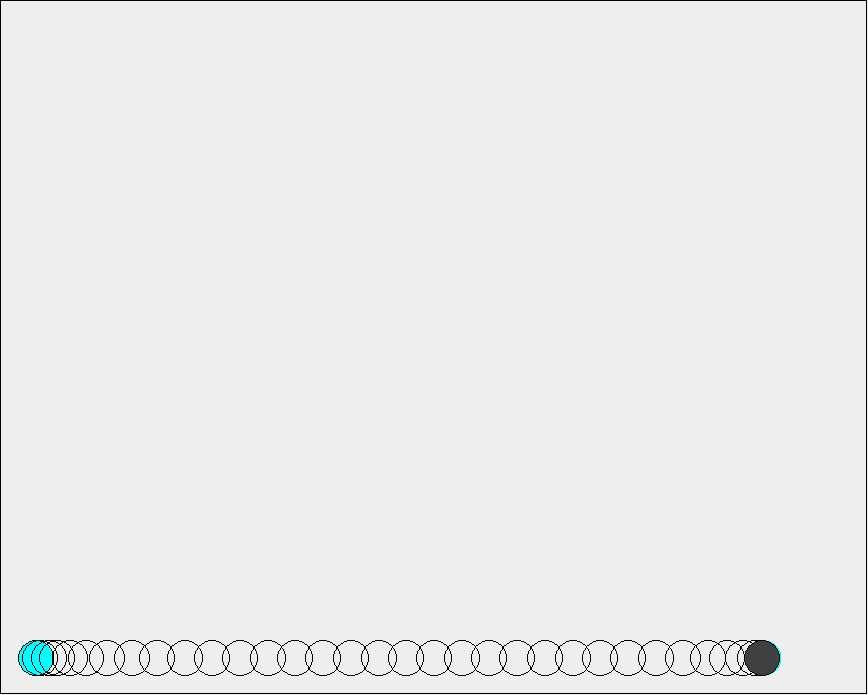
\includegraphics[width=\textwidth]{bench-0}
        		\caption{Up/Down 0}
        		 \label{fig:bench-0}
	\end{subfigure}	
	\hfill
	\begin{subfigure}[t]{0.3\columnwidth}
        		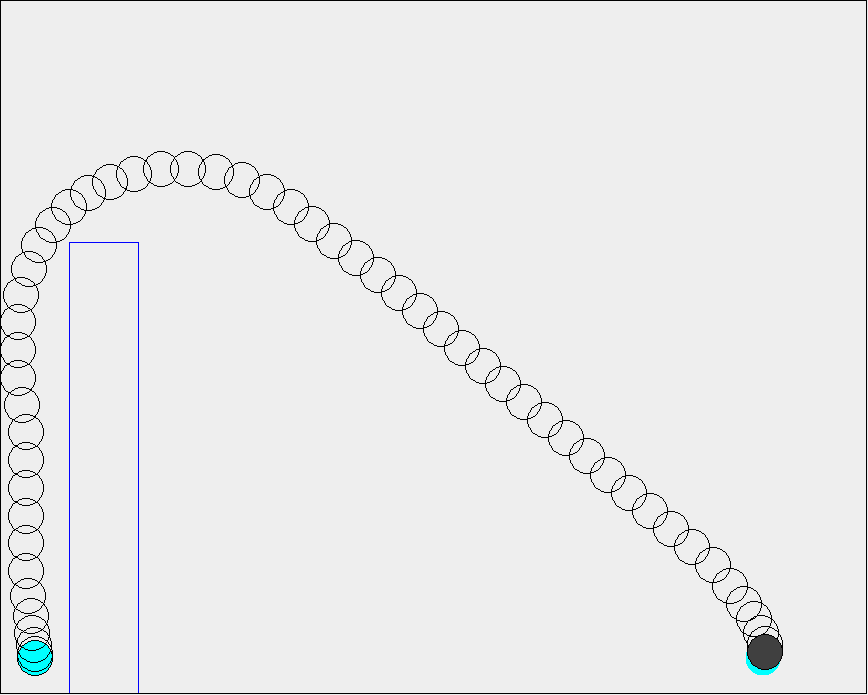
\includegraphics[width=\textwidth]{bench-1}
        		\caption{Up/Down 1}
        		 \label{fig:bench-1}
	\end{subfigure}	
	\hfill
	\begin{subfigure}[t]{0.3\columnwidth}
        		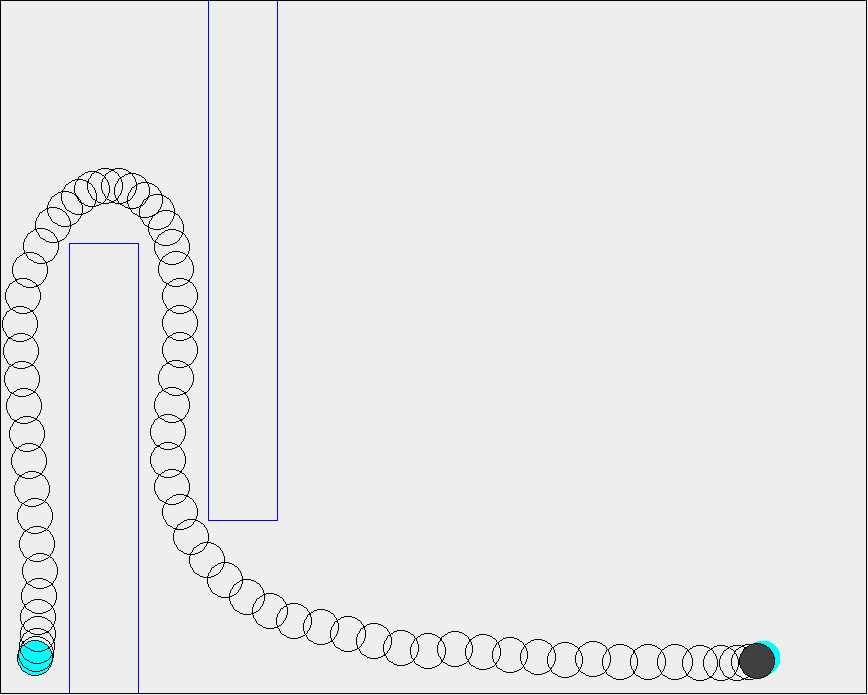
\includegraphics[width=\textwidth]{bench-2}
        		\caption{Up/Down 2}
        		 \label{fig:bench-2}
	\end{subfigure}
%	\par\bigskip
	\begin{subfigure}[t]{0.3\columnwidth}
        		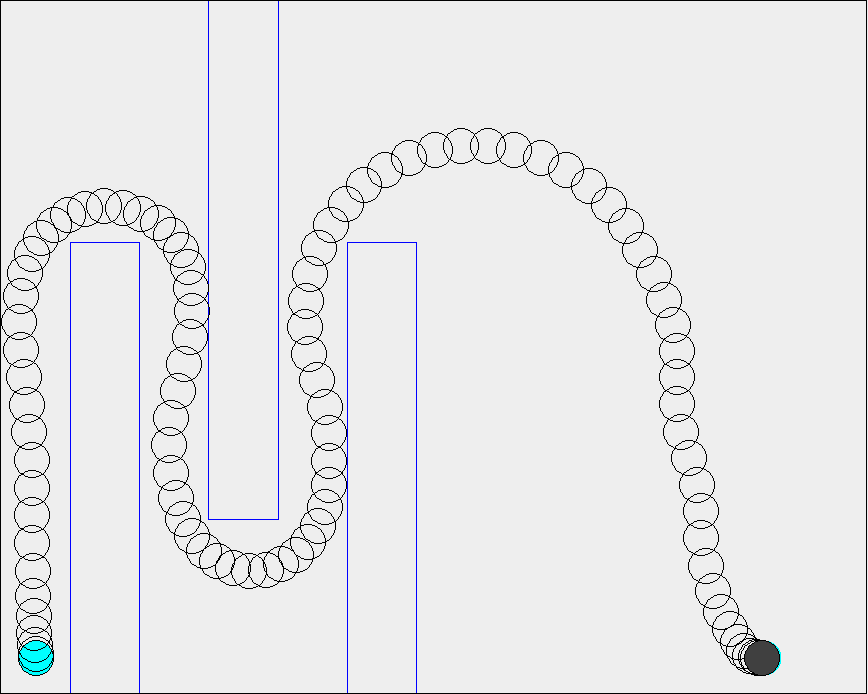
\includegraphics[width=\textwidth]{bench-3}
        		\caption{Up/Down 3}
        		 \label{fig:bench-3}
	\end{subfigure}	
	\hfill
	\begin{subfigure}[t]{0.3\columnwidth}
        		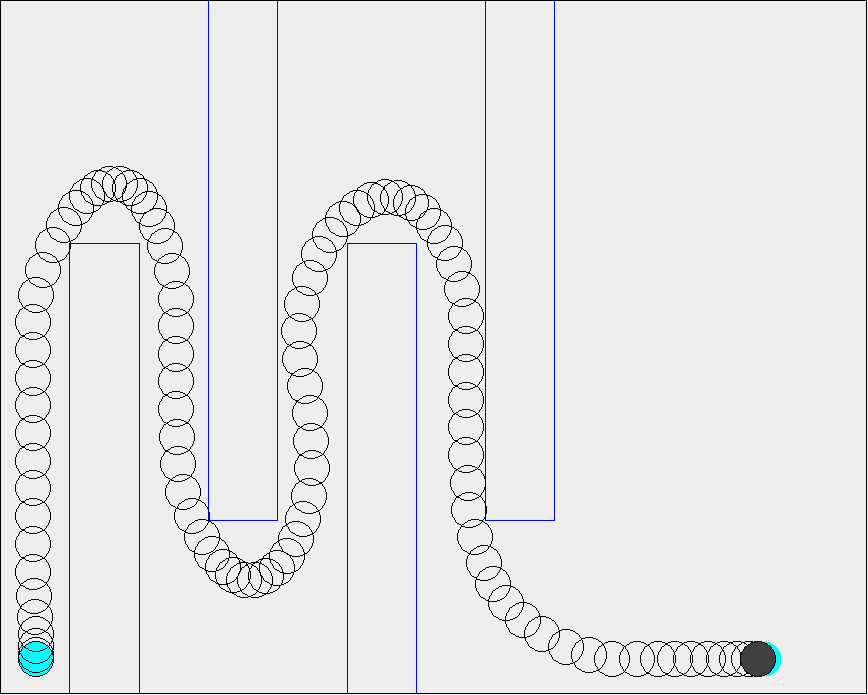
\includegraphics[width=\textwidth]{bench-4}
        		\caption{Up/Down 4}
        		 \label{fig:bench-4}
	\end{subfigure}	
	\hfill
	\begin{subfigure}[t]{0.32\columnwidth}
        		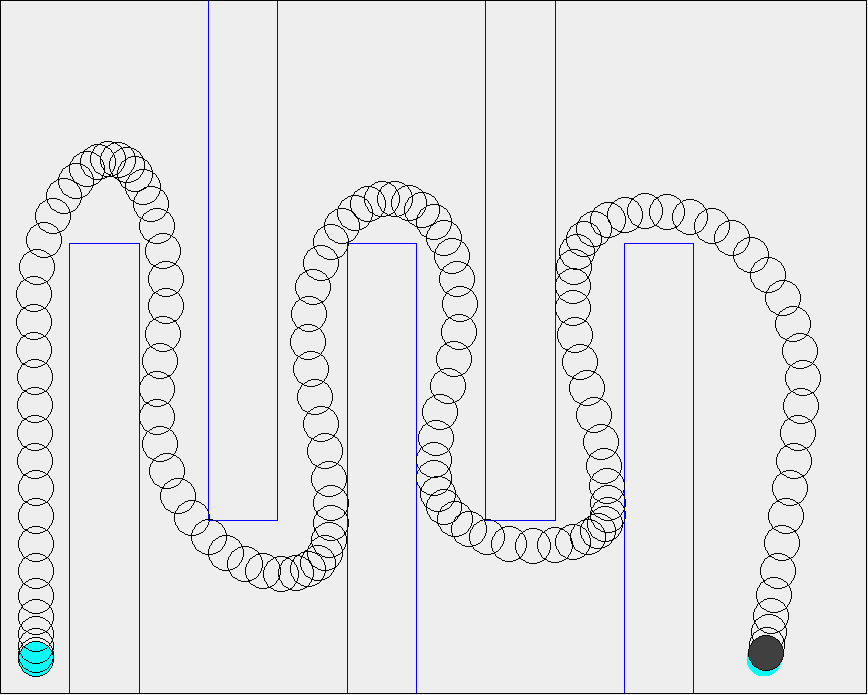
\includegraphics[width=\textwidth]{bench-5}
        		\caption{Up/Down 5}
        		 \label{fig:bench-5}
	\end{subfigure}		
	
			
	\caption[The six variations of the Up/Down scenario]{The six variations of the Up/Down scenario, ranging from no obstacles in \ref{fig:bench-0} to five obstacle in \ref{fig:bench-5}.}
    \label{fig:bench-pure}     
\end{figure}
In the experiment, the UAV must move from a point in the bottom-left corner of the world to a point in the bottom-right corner. Six different scenarios are tested. The different scenarios have a varying amount of rectangular obstacles in their world, ranging from zero at all to five obstacles. These obstacles are laid out in such a way that the UAV must zig-zag up and down to reach its goal. The time step size is $0.2s$, and there are 30 seconds worth of time steps modeled in scenario. 
\par
Figure \ref{fig:bench-pure} shows the different scenarios and the trajectory found as the solution for that scenario. Figure \ref{fig:pure-data} shows a graph of the trajectory scores, measured in seconds. The trajectory score is the time it takes for the UAV to reach its goal when it follows that trajectory. It also shows the execution time. Each scenario was executed 5 times, and execution time was limited to 900 seconds.

\begin{figure}[t]
	\centering
	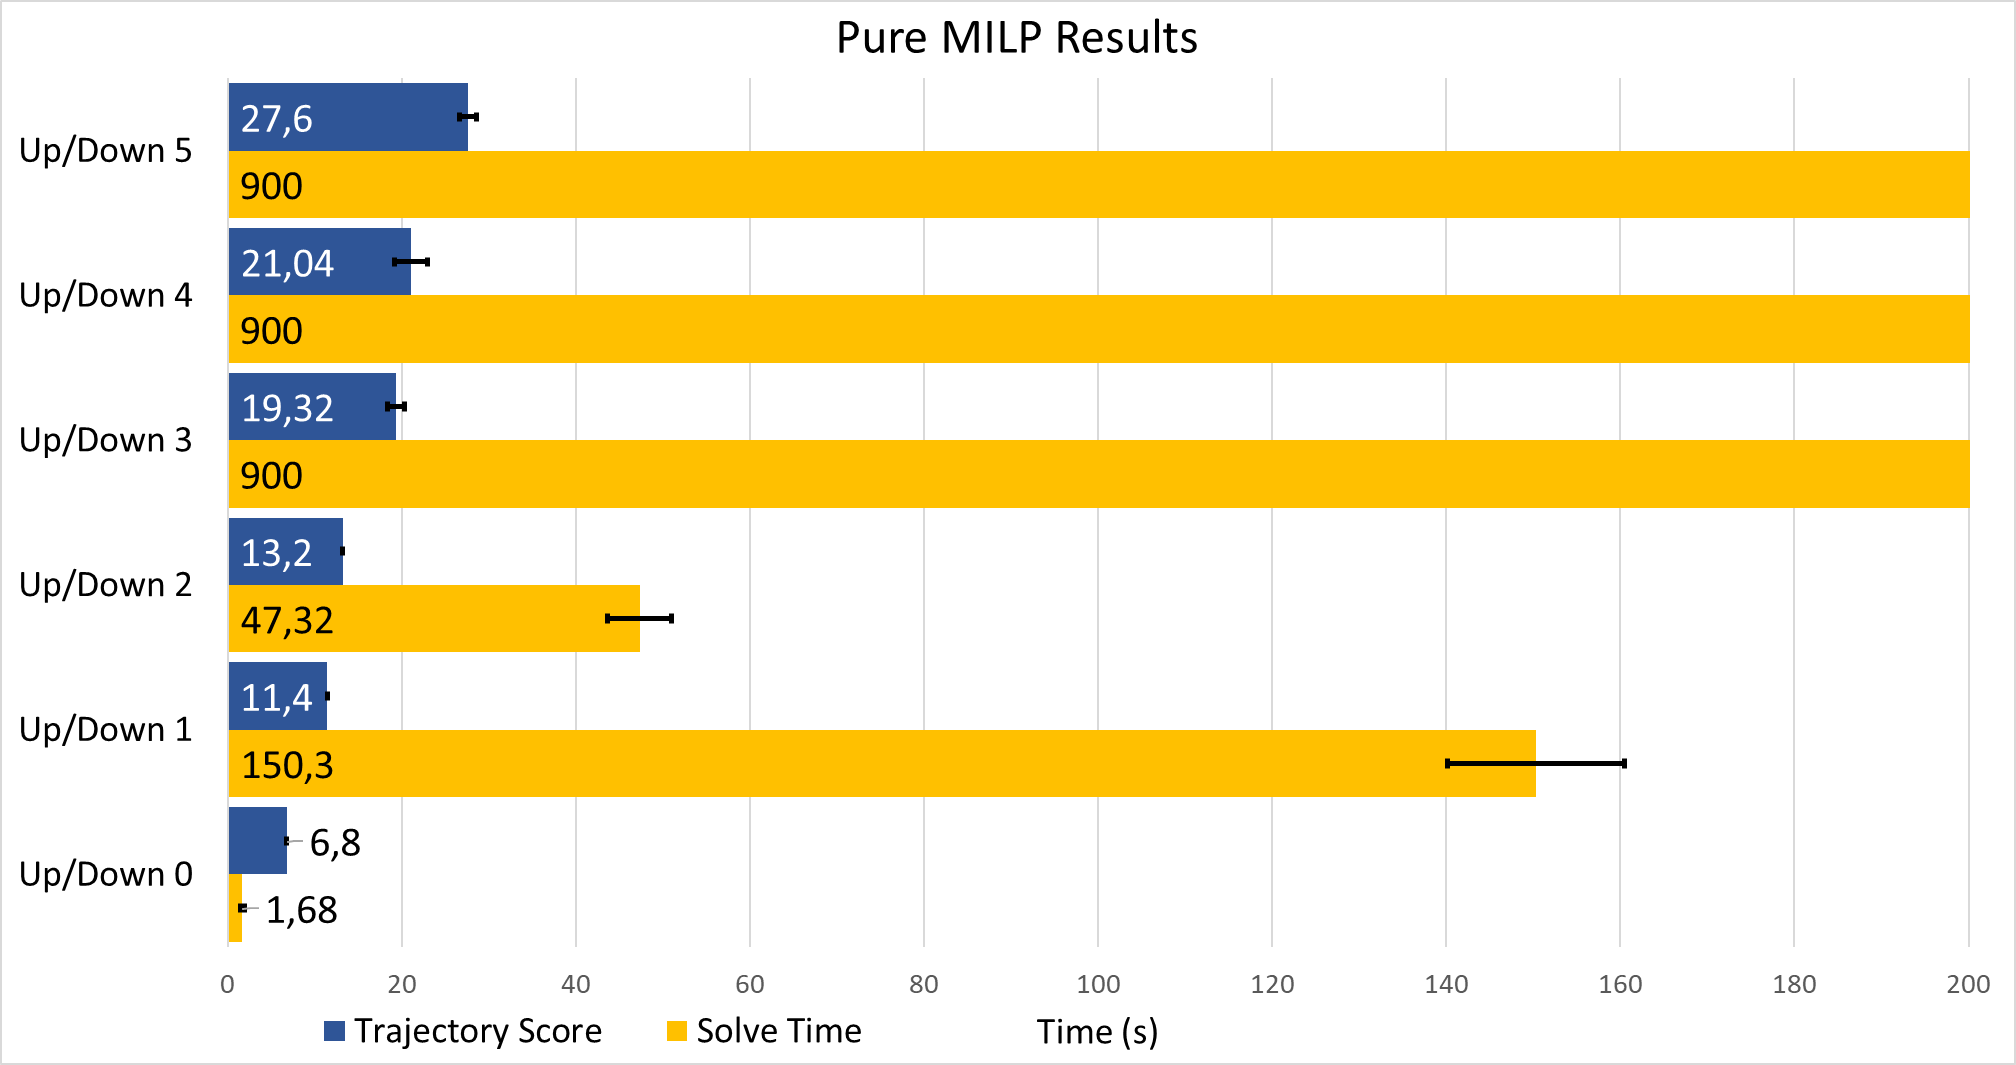
\includegraphics[width=\textwidth]{pure-milp-data}
	\caption[The results for the pure MILP approach ]{The results of the Up/Down scenario for the pure MILP approach with varying numbers of obstacles. The error bars show the 95\% confidence interval.}
	\label{fig:pure-data}
\end{figure}

Without any obstacles, the solver finds the trajectory in under two seconds. However, when even a single obstacle is added, the solver needs more than two minutes to find the optimal trajectory. When another obstacle is added, the solve time drops to below a minute again even though there are more integer variables used in the model. Starting at three obstacles and more, the solver can no longer find the optimal trajectory in less than 15 minutes. Clearly, this is not going to scale well to large scenarios.
\section{Algorithm approach}
Mixed-Integer programming belongs to the ``NP-Complete'' class of problems \cite{DBLP:conf/coco/Karp72}. Assuming there are $n$ boolean variables, the worst case time complexity is $O(2^n)$. A boolean variable is needed for every edge of every polygon, for every time step. By reducing both the amount of time steps needed and the amount of obstacles that need to be modeled, the solve time can be reduced dramatically. \\
The key insight that allows my algorithm to scale well beyond what's usually possible is that the trajectory planning problem does not need to be solved all at once. If the trajectory planning problem can be split into many different subproblems, each subproblem becomes easier to solve. The solution for each subproblem is a small part of the final trajectory. By solving these subproblems sequentially, the final trajectory can gradually be constructed. \\
While splitting the problem into subproblems does make each subproblem much easier to solve, it also has an important down side: finding the fastest trajectory can no longer be guaranteed. Smaller subproblems make it easier to find a solution, but fundamentally the problem of finding the optimal trajectory is still just as hard. The necessary trade-off for better performance is that the optimal trajectory will likely not be found. Luckily, the optimal trajectory is often not required in navigation. A reasonably good trajectory will do.

\subsection{Importance of convexity}
The worst case time needed to solve a MILP problem increases exponentially with the amount of integer variables. However, this is not the most useful way to measure the difficulty of a problem. Modern solvers are heavily optimized and are able to solve certain problems with many integer variables much faster than others. The key difference is the convexity of the solution space. Just like a circle is the solution space for ``all points a certain distance away from the center point'', the constraints used to model the trajectory planning problem form some geometric shape with a dimension for every variable. \\
When only linear constraints with real values are allowed, the solution space will always be convex. It is this convexity that makes a standard linear program easy to solve. When integer variables are introduced, it is possible to construct solution spaces which are not convex. As the solution space becomes less and less convex, the problem becomes harder to solve. Integer variables can be seen as a tool which allows non-convex solution spaces to be modeled. When trying to improve the difficulty of a problem, the actual goal is making the problem more convex (or smaller, which always helps). Reducing the amount of integer variables is only a side effect. \\
This insight is critical when determining how to divide the trajectory problem into smaller subproblems, and which obstacles are important for each subproblem.
\newpage
\begin{algorithm}[t]
\caption{General outline}
\label{alg:outline}
\begin{algorithmic}[1]
\State $T \leftarrow \{\}$ \Comment{The list of solved subtrajectories}
\State $path \leftarrow$ \Call{Theta*}{$scenario$}
\State $events \leftarrow$ \Call{FindTurnEvents}{$path$}
\State $segments \leftarrow$ \Call{GenSegments}{$path$, $events$}
\ForEach {$segment \in segments$}
\State \Call{UpdateStartState}{$segment$}
\State \Call{GenSafeRegion}{$scenario$, $segment$}
\State \Call{GenSubMILP}{$scenario$, $segment$}
\State $T \leftarrow T \cup \{$ \Call{SolveSubMILP}{} $\}$
\EndFor
\State $result \leftarrow $\Call{MergeTrajectories}{$T$}
\end{algorithmic}
\end{algorithm}

\subsection{General Algorithm Outline}
Algorithm \ref{alg:outline} shows the general outline of the algorithm. It consists of two phases. The first phase gathers information about the trajectory planning problem. A Theta* path planning algorithm is used to find an initial path (line 2). Unlike a trajectory, a path is time-independent and does not take the UAV's dynamics into account. From this initial path, turn events are generated (line 3). These turn events mark where the trajectory will have to turn. \\
The second phase builds and solves "segments". Each segment represents a single sub-trajectory. The segments contain the information needed to build the corresponding MILP subproblem, which can in turn be solved by the solver to find the sub-trajectory. First, each segment is generated (line 3) from the turn events found in the previous step. Before the MILP sub-problem can be generated and solved (line 8-9), a heuristic selects several obstacles to be modeled in the problem. A genetic algorithm generates a safe region which is allowed to overlap those selected obstacles only (line 7). To ensure a seamless transition between two consecutive sub-trajectories, the starting state for the UAV in the MILP problem for the current segment is updated to match the final state of the UAV in the previous segment (line 6). Finally, the sub-trajectories are merged together to form the final trajectory (line 11).

\section{Finding the initial path}
\label{subsec:initial-path}
The first step in Algorithm \ref{alg:outline} is finding the Theta* path (line 2). This path will be used to split the trajectory planning problem into segments. The MILP problem generated from each of those segments needs an intermediate goal to get the UAV closer to the final goal position. These intermediate goals will be determined by the Theta* path. \\
This path is not only useful to guide the trajectory towards the goal. It also lets the algorithm determine where the turns will be in the trajectory, since the turns in the trajectory will match the turns in the Theta* path.

\subsection{A*}
Theta* is a variant of the A* path planning algorithm. In A*, the world is represented as a graph. Each possible position is represented as a node in that graph, with edges between nodes if one position can be reached from the other. The distance between connected positions is represented as a weight or cost on each edge. \\
Planning a path consists of picking a start and goal node. The A* algorithm will traverse the edges between nodes, keeping track of which edges it traversed to reach a certain node. When the algorithm reaches the goal node, the nodes visited to reach that goal node are the path from the start node to the goal . \\
In this thesis, the world the UAV travels through is a continuous (2D) world. The graph for A* is generated by overlaying a grid on the world. Nodes are placed at each intersection of the grid, as long as they are not inside obstacles. Each node is also connected to its neighbors by moving horizontally, vertically or diagonally along the grid. Figure \ref{fig:astar-grid} shows an example of this.
\begin{figure}
\centering
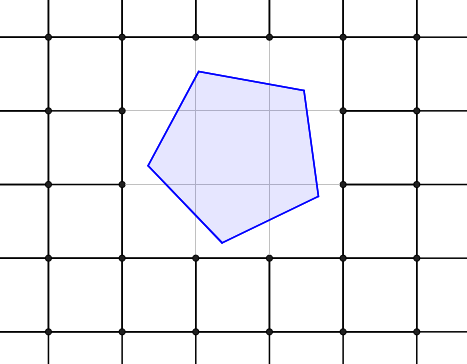
\includegraphics[width=0.5\textwidth]{astar-grid}
\caption[The grid used to build the graph for the Theta* algorithm]{An example of how a grid is used to build the graph for the path finding algorithm. Each point is a node on the graph. If two points are connected by a line, their nodes in the graph also are connected by an edge. Diagonal edges are not shown here for clarity.}
\label{fig:astar-grid}
\end{figure}

\begin{figure}[h]
\centering
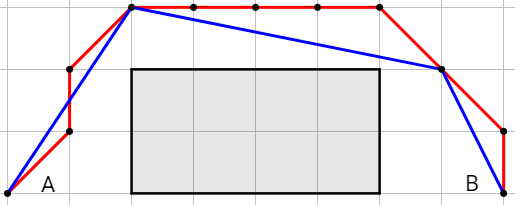
\includegraphics[width=0.5\textwidth]{a_theta_star_comp3}
\caption[A comparison between an A* and Theta* path]{The red line shows a typical A* path, compared to the path found by Theta*. The gray rectangle is an obstacle.}
\label{fig:thetastarcompare}
\end{figure}

\subsection{Reason for Theta*}
A* finds the shortest path through the graph. However, this graph is only an approximate representation of the actual continuous world. An A* path will only travel along the edges of the graph. This means that the path can only travel horizontally, vertically and possibly diagonally. If the shortest path between two points is at another angle, the A* path will contain zig-zags or detours because it is limited to traveling along the grid. \\
Theta* solves this problem. It is nearly identical to A*, but it allows the path to travel at arbitrary angles. It still traverses the graph using the edges between nodes, but does not restrict the path to only following those edges. Figure \ref{fig:thetastarcompare} shows the effect of this change.




\subsection{Theta* implementation}

Theta* was originally developed by Daniel et al. \cite{Daniel2010}. This section, including Algorithm \ref{alg:thetastar}, paraphrases their excellent explanation of the algorithm. The implementation is shown in Algorithm \ref{alg:thetastar}, which uses the following elements:
\begin{itemize}
\item The g-value $g(s)$ is the length of the shortest path between the start node and $s$.
\item A function $c(s,s')$ which returns the distance between node $s$ and $s'$.
\item A heuristic function $h(s)$, which approximates the path distance left before the goal position $s_{goal}$ is reached. The straight line distance between $s$ and the $s_{goal}$ is used, such that $h(s) = c(s,s_{goal})$. An admissible heuristic function must always be an underestimation of the actual path distance to the goal, which is ensured by using the straight line distance. 
\item A function $parent(s)$ which returns the node before $s$ in the path. When the parent of a node is $null$, it is either not part of the path or the first node of the path.
\item A priority queue $queue$. This is a queue of nodes to expand next. Each node $s$ is added with a value $x$ using the $queue.$Insert($s$,$x$) method. If $s$ is already in $queue$, its value is updated to $x$. The $queue$.Pop() method removes and returns the node $s$ with the lowest value $x$.
\item A set $expanded$ which contains all nodes which have already been expanded.
\item A function GenerateNeighbors($s$) which generates and returns the neighbors of node $s$. These are the neighboring positions on the grid around $s$
\end{itemize}

\begin{algorithm}[h]
\caption{Theta* Implementation}
\label{alg:thetastar}
\begin{algorithmic}[1]
\Function{Theta*}{$scenario$}
	\State $g(v_{start}) \leftarrow 0$
	\State $parent(v_{start}) \leftarrow null$
	\State $queue \leftarrow \emptyset$
	\State $queue$.Insert($v_{start}$, $g(v_{start}) + h(v_{start})$)
	\State $expanded \leftarrow \emptyset$
	\While{$queue \neq \emptyset$}
		\State $s \leftarrow queue$.Pop()
		\If{$s = v_{goal}$}
			\Return $s$.GetPath()
		\EndIf
		\State $expanded \leftarrow expanded \cup \{s\}$
		\ForEach{$s' \in ~ $GenerateNeighbors($s$)}
			\If{$s' \notin expanded $}
%				\If{$s' \notin queue$}
%					\State{$g(s') \leftarrow \infty $}
%					\State{$parent(s') \leftarrow null $}
%				\EndIf
				\State{UpdateVertex($s$,$s'$)}
			\EndIf
		\EndFor
	\EndWhile
	\Return "no path found"
\EndFunction
\Function{UpdateVertex}{$s$,$s'$}
	\If{LineOfSight($parent(s)$,$s'$)}
		\State $s_{parent} \leftarrow parent(s)$
	\Else
		\State $s_{parent} \leftarrow s$	
	\EndIf
	\If{$g(s_{prev}) + c(s_{prev},s') < g(s')$}
		\State $g(s') \leftarrow g(s_{parent}) + c(s_{parent},s')$
		\State $parent(s') \leftarrow s_{parent}$
		\State $queue$.Insert($s'$,$g(s') + h(s')$)
	\EndIf
\EndFunction{}
\end{algorithmic}
\end{algorithm}
\paragraph{Initialization}
When the algorithm initializes, the g-value of the start node $v_{start}$ is set to zero and its parent is set to $null$ (line 2-3). The priority queue $queue$ is initialized, and $v_{start}$ is added to it with value $g(v_{start}) + h(v_{start})$. The value attached to a node $v$ in the priority queue is the shortest possible length of a path going from the start $v_{start}$ to the goal $v_{goal}$, while going through $v$. The g-value is the length of the path between $v_{start}$ and $v$, while $h(s)$ is an estimate of the length of the path between $v$ and $v_{goal}$.
\paragraph{Main loop}
$queue$.Pop() always removes the node $s$ with the lowest value (line 8). This means that as more nodes get added to $queue$, the algorithm will always explore the "most promising leads" first. If $s = v_{goal}$, the goal has been reached and the path is returned (line 9-11). Otherwise, $s$ is added to $expanded$ (line 12). This prevents $s$ from being added to $queue$ again. Line 13 generates every neighbor $s'$ of $s$ according to the grid and obstacles, as seen in Figure \ref{fig:astar-grid}, "expanding" node $s$. If the neighbor $s'$ has not been expanded yet, UpdateVertex($s$,$s'$) is called (line 14-16).
\paragraph{UpdateVertex}
So far, the algorithm is identical to A*. The only difference between A* and Theta* are lines 22-26. Line 22 checks if the parent of $s$, which is the node before $s$ in the path, can be connected in a straight line to $s'$. Going from $parent(s)$ to $s'$ directly is always shorter than going from $parent(s)$ to $s$ and from $s$ to $s'$ due to the triangle inequality. If $parent(s)$ and $s'$ are in line of sight, the path should be constructed from $parent(s)$ to $s'$, skipping $s$. Otherwise, the path goes through $s$, which is the behavior  of A*. The choice of which node should be the parent of $s'$ is stored as $s_{parent}$\\
Line 27 checks if the path through $s_{parent}$ to $s'$ is the shortest path to $s'$ found so far. If this is not the case, a shorter path to $s'$ exists so the  path through $s_{parent}$ can safely be ignored. Otherwise, the g-value of $s'$ is updated to the length of the path to $s_{parent}$, $g(s_{parent})$ plus the distance between $s_{parent}$ and $s'$, $c(s_{parent},s')$ (line 28). The shortest path to $s'$ is updated by setting $parent(s')$ to $s_{parent}$ (line 29). Finally, $s'$ is added to $queue$ to be expanded further.
\subsection{Performance improvements}
By introducing the line of sight check, Theta* is considerably slower than A* in large worlds with many obstacles. The goal of this thesis is to improve scalability of trajectory planning to large and complex worlds, so the preprocessing phase must also scale well. \\
To help Theta* scale better, the world is divided into rectangular sectors. When the world is first loaded, the algorithm determines in which sector(s) each obstacle is placed, creating an index mapping sectors to obstacles. \\
When the line of sight check is executed, the algorithm determines which sectors the line crosses. This is usually just one or two sectors. By using the index, only the obstacles in those sectors need to be considered for the line of sight check. This is much faster than having to check every obstacle in the entire world every time.



\section{Detecting turn events}
\label{subsec:corner-events}
%According to Hypothesis \ref{hyp:nonconvex}, the degree of non-convexity around the trajectory is responsible for the poor performance of MILP trajectory planning problem. This local degree of non-convexity around the trajectory is the amount of distinct convex shapes the trajectory needs to pass through to reach the goal position, such that every point in the trajectory lies within at least one shape. \\
%Within a single convex shape, by definition, it is always possible to move in a straight line from one side of the shape to the other. As a consequence, if multiple convex shapes are needed, the trajectory needs to make a turn. If the turn is not needed, that implies the trajectory can go in a straight line, which means that only a single convex shape is needed. \\
%Because of this, the turns in the trajectory and the degree of non-convexity are  directly related. Every turn in the trajectory is a manifestation of a transition between two or more convex shapes, and thus contributes to the degree of non-convexity of the entire trajectory. \\
%Solving the trajectory in smaller segments reduces the degree of non-convexity in each segment, making them easier to solve. If Hypothesis \ref{hyp:nonconvex} is true, minimizing the amount of turns in each segment will improve performance even more. \\
%While the Theta* path is only a rough approximation of the trajectory, it does have turns in roughly the same places as the trajectory will have. Finding those turns allows the algorithm build segments such that the amount of turns in each segment is minimal. \\
%Because Theta* is used to generate the initial path, finding the turns is easy. When two nodes are in each other's line of sight, it is possible to construct a convex shape around those points. When they are not within line of sight, which is when Theta* keeps the previous node in the path, this is not possible. Using the same reasoning as above, the nodes in the Theta* path must always coincide with turns in both the Theta* path and the trajectory. \\






%With an initial path generated, the next problem is dividing it into segments. Dividing the path into equal parts presents problems, because when solving each segment, the solver has no knowledge of what will happen in the next segment. This is especially problematic when the vehicle needs to make a tight corner. If the last segment ends right before the corner, it may not be possible to avoid a collision. Because of this, corners need to be taken into account when generating the segments. The right image in figure \ref{fig:pre-1-2} shows the transitions between segments as green circles.\\
%In Euclidian geometry, the shortest path between two points is always a straight line. When polygonal obstacles are introduced between those points, the shortest path will be composed of straight lines with turns at one or more vertices of the obstacles. The obstacle that causes the turn will always be on the inside of the corner. This shows why corners are important for another reason: They make the search space non-convex. For obstacles on the outside of the corner it is possible to constrain the search space so it is still convex, but this is not possible for obstacles on the inside of a corner.\\
%Because of these reasons, isolating the corners from the rest of the path is advantageous. With enough buffer before the corner, the vehicle is much more likely to be able to navigate the corner successfully. It also means that the computationally expensive parts of the path are as small as possible while still containing enough information for fast navigation through the corners.
%\\
%The reason for using Theta* becomes clear now. Every single node in the path generated by the algorithm is guaranteed to be either the start, goal or near a corner. A corner can have more than one node, so nodes which turn in the same direction and are close to each other are grouped together and considered part of the same corner. For each corner, a corner event is generated.

The initial Theta* path shows the direction in which the UAV has to move to reach the goal. The next step is generating segments along this path. These segments will be solved to build the trajectory for the UAV. The segments are generated around the turns in the Theta* path. There are two reasons for this.
\par
\begin{figure}
\centering
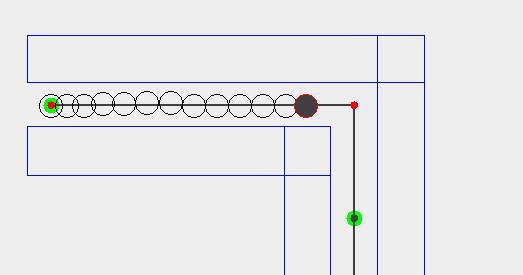
\includegraphics[width=0.65\textwidth]{small-margin-fail-post}
\caption[An example of the UAV going too fast to execute a turn]{The  UAV, represented as the filled black circle, at a transition between segments. It ended the previous segment (on the left) with a high velocity. It cannot slow down in time to turn the corner without a collision.}
\label{fig:turn-fail}
\end{figure}
The first reason is that it helps ensure that each segment can always be solved. When the UAV reaches the goal of a specific segment, it may be traveling at a high velocity. This means that it may also start the next segment at a high velocity. If this transition between segments happens right before a tight corner, the UAV may not be able to avoid a collision in the segment it is transitioning to. This is shown in Figure \ref{fig:turn-fail}.
\par
\begin{figure}
\centering
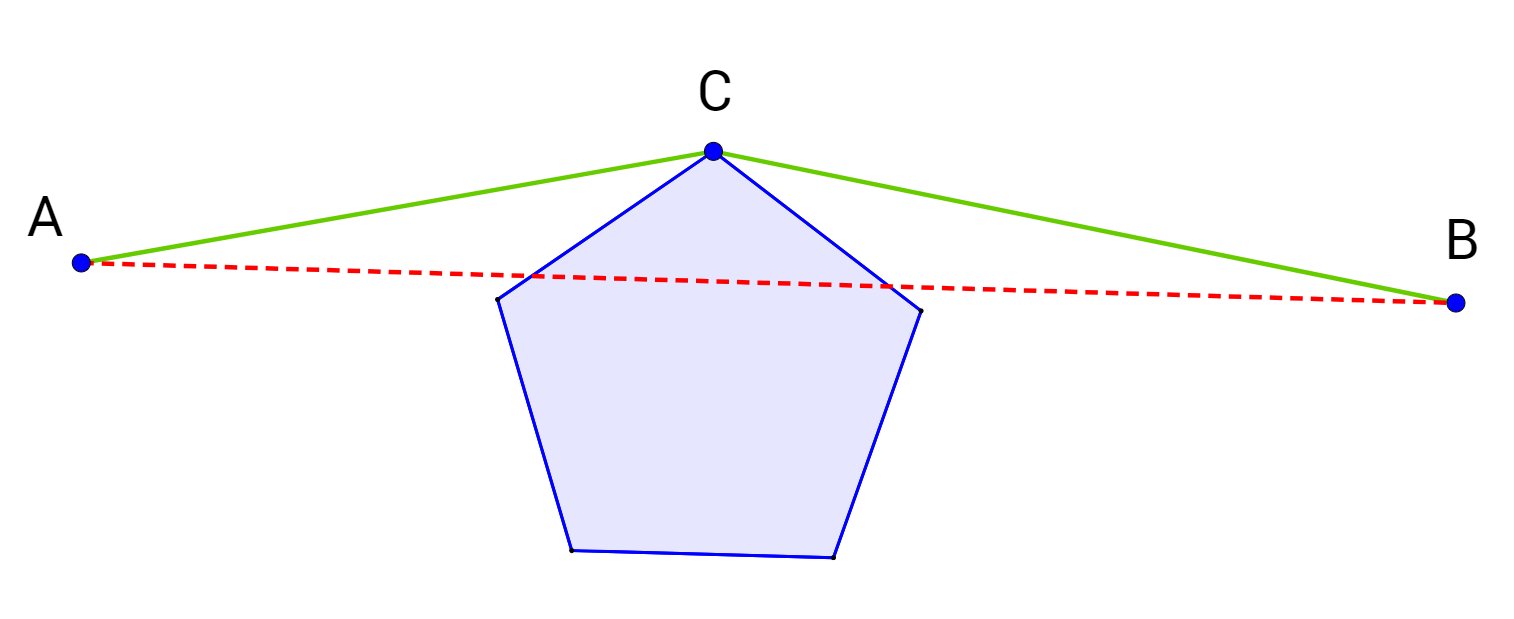
\includegraphics[width=0.65\textwidth]{inside-corner}
\caption[A demonstration of how obstacles cause turns]{The straight line path between A and B (red dashed line) is not possible because the blue obstacle is in the way. The shortest path now passes through point C (green line). The blue obstacle causes the turn in point C to exist.}
\label{fig:inside-corner}
\end{figure}
The second reason is that generating the segment around turns in the Theta* path helps improve performance. In Euclidian geometry, the shortest path between two points is always a straight line. When polygonal obstacles are introduced between those points, the shortest path will be composed of straight lines with turns at one or more vertices of the obstacles. The obstacle that causes the turn will always be on the inside of the corner. This is shown in Figure \ref{fig:inside-corner}.
\par
Turns in the Theta* path are also expressions of non-convex parts in the problem. Looking at Figure \ref{fig:inside-corner} again, points A and B are both valid positions in the search space. However, because the red line passes through an obstacle, the search space is non-convex. The red line crossing the obstacle causes both the turns and the non-convex search space. Therefore, the turns in the Theta* path can be seen as manifestations of the non-convexity of the search space.
\par
Since poor performance of any MILP is due to the non-convexity of the search space, the individual subproblems should be kept as convex as possible. By generating the segments around these turns, the algorithm can ensure that there is at most one turn per segment. This limits the non-convexity in the subproblem defined by each segment.
\par
While every node in the Theta* path (except the start and goal) coincide with a turn, they can be close together. When two or more consecutive nodes turn in the same direction (clockwise or counter-clockwise) and are close enough together, they can be considered to represent a single turn. The algorithm groups those nodes together in a turn event. Each turn event contains one or more nodes. A turn event predicts the existence of a turn in the MILP trajectory based on the   Theta* path, bridging the gap between them. This is demonstrated in Figure \ref{fig:turn-events}.

\begin{figure}
\centering
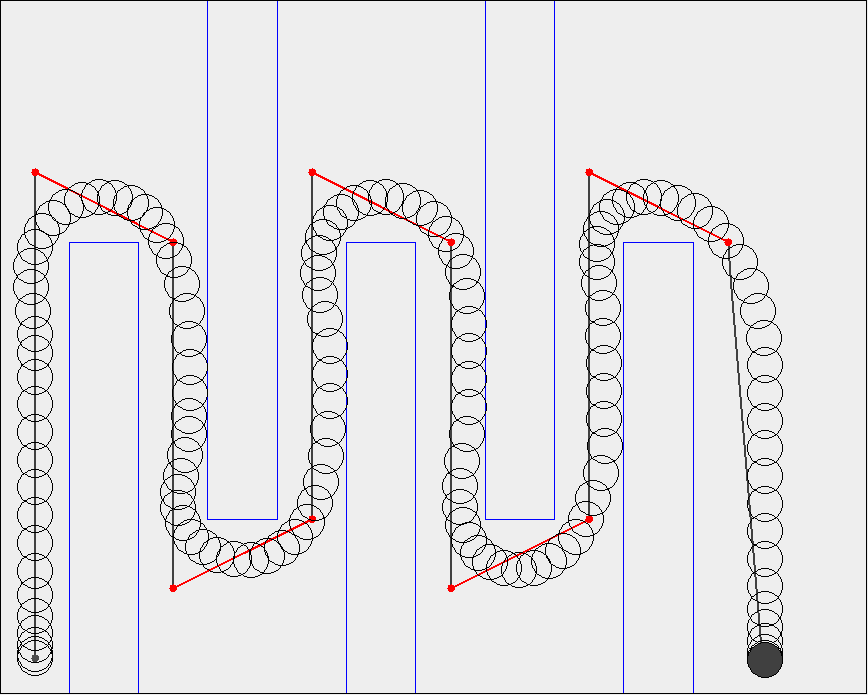
\includegraphics[width=0.65\textwidth]{turn-events}
\caption[A visualization of turn events]{This figure shows the Theta* path on the Up/Down scenario, with the turn events on that Theta* path highlighted in red. The trajectory of the UAV is also shown to illustrate how the turn events on the Theta* path match up with turns in the trajectory.}
\label{fig:turn-events}
\end{figure}
\newpage
\begin{algorithm}[t]
\caption{Finding Turn Events}
\label{alg:corners}
\begin{algorithmic}[1]
\Function{FindTurnEvents}{$path$}
  \State $\Delta max \leftarrow$ max. acc. distance * turn tolerance
  \State $events \leftarrow \{\}$ \Comment{The list of turn events found so far}
  \State $i \leftarrow 1$ \Comment{Skip the start node, it can't be a turn}
  \While{$i < |path| - 1$ } \Comment{Skip the goal node}
  	\State $event \leftarrow \{ path(i) \}$ \Comment{Start new turn event}
  	\State $turnDir \leftarrow$ \Call{TurnDir}{$path(i)$} 
    	\State $i \leftarrow  i + 1$
    	\While{$i < |path| - 1$ }
    	\If{$||path(i-1) - path(i)|| > \Delta max$}
    		\Break \Comment{Node is too far from previous}
	\EndIf
	\If{\Call{TurnDir}{$path(i)} \neq turnDir$}
		\Break \Comment{Node turns in wrong direction}
	\EndIf
	\State $event \leftarrow event \cup \{ path(i) \}$\Comment{Add to event}
	\State $i \leftarrow  i + 1$
	
    	\EndWhile
    	
    	\State $events \leftarrow events \cup \{ event \}$
  \EndWhile
\Return $events$
\EndFunction
\end{algorithmic}
\end{algorithm}

\subsection{Algorithm Implementation}
Algorithm \ref{alg:corners} processes the Theta* path to generate turn events. Two factors determine whether or not nodes are grouped together into events:
\begin{itemize}
\item The turn direction: a node $v$ in the path can either turn the path clockwise or counter-clockwise, as determined by TurnDir($v$) Two nodes with a different turn direction cannot be in the same turn event.
\item The maximum distance between two nodes in a turn event: Nodes which are too far from each other should not be merged. This distance $\Delta max$ is based on a turn tolerance parameter multiplied by the UAV's maximum acceleration distance (MAD). 
\end{itemize}



\paragraph{Maximum Acceleration Distance}
With $a_{max}$ and $v_{max}$ respectively the UAV's maximum acceleration and velocity, the time needed to reach the maximum velocity is $t_{max} = v_{max} / a_{max}$. The maximum acceleration distance is the distance traveled during that time, which equals $t_{max}^2 / 2 = v_{max}^2 / 2a_{max}$. The $MAD$ is used in several places in the algorithm as an approximation of the distance in which the UAV can recover from a maneuver. In $1*MAD$, the UAV can accelerate to any velocity from zero, or it can stop from any velocity. In $2*MAD$, the UAV can transition from any velocity vector to any other velocity vector. It is an approximation of the distance at which the presence or absence of an event can influence the UAV. \\
In this case, the MAD is relevant because turns require the velocity vector of the UAV to change from their value before the turn to a new value after the turn. If two nodes have a distance of more than $2*MAD$ between them, the turns at each node can be handled independently as distinct turns. 
\par
In the Theta* path, all but the first and last nodes are turns in the path. The second node is always the first node in a new turn event (line 5). Subsequent nodes in the path which are not too far away from the previous node (line 9) and turn in the same direction (line 12) are added to the current turn event (line 15). The maximum distance between nodes in the same turn is $\Delta max$. Once a node is found which does not belong in the event, the event is stored (line 18), a new event is created for that node (line 5) and the process repeats until no more nodes are left.


\section{Generating path segments}

Once the turn events are found, the next step is generating the segments. Each segment defines a single MILP problem whose solution is a small part of the desired trajectory. Every segment should contain at most one turn event to keep solve times low.\\
The boundaries of the segments are calculated based on the Theta* path and the turn events. For the best performance, these segments should be as small as possible. However, performance is not the only factor. Stability of the algorithm is also important. Each segment needs to be large enough so the UAV can safely approach and exit each turn. This can be guaranteed by ensuring that the start of a segment is always at least the maximum acceleration distance (MAD) before the turn event. The distance between the start of the segment and the turn event in that segment is called the expansion distance. When the expansion distance is at least $1*MAD$, the UAV can come to a complete stop before it reaches the turn. If the UAV can safely come to a stop, it can also slow down to an appropriate velocity to safely navigate the turn. Extending the segment beyond the end of the turn event also ensures that the UAV must have completely navigated the turn by the end of the segment. Ensuring that the UAV can always safely navigate a turn means that the MILP solver can always find a feasible trajectory for that segment. Because of this, ensuring  safety also ensures stability of the algorithm. \\
Increasing the approach margin beyond the minimum required for stability can improve the speed of the trajectory. An approach margin of $1*MAD$ is considered safe because the UAV can still "slam on the breaks" to slow down in time for the turn. However, a larger expansion distance gives the UAV more time and space to maneuver so it can efficiently navigate the turn. The ratio between the expansion distance and the $MAD$ is called the approach margin: $expansion distance = approach margin * MAD$. Since the $MAD$ is determined by the UAV's properties, the approach margin is used as the parameter which controls the expansion distance.


\begin{algorithm}[h]
\caption{Generating the segments}
\label{alg:segments}
\begin{algorithmic}[1]
\Function{GenSegments}{$path$, $events$}
\State $segments \leftarrow \{\}$
\State $catchUp \leftarrow true$
\State $lastEnd \leftarrow path(0)$
\For {$i \gets 0, |events| - 1 $}
\State $event \leftarrow events(i)$
\If{$catchUp$}
	%\State $segStart \leftarrow $ \Call{ExpandBackw}{$event.start$}
	%\State \Call{AddSegments}{$lastSegEnd$, $segStart$}
	%\State $lastSegEnd \leftarrow segStart$
	\State \Call{ExpandBackwards}{$event.start$} 
	\State \Call{AddSegments}{$lastEnd$,$event.start$}
	\State $lastEnd \leftarrow event.start$
\EndIf
\State $nextEvent \leftarrow events(i+1)$
\If{$nextEvent.start$ is close to $event.end$}
	\State $mid \leftarrow$ middle between $event$ \& $nextEvent$
	\State \Call{AddSegments}{$lastEnd$,$mid$}
	\State $lastEnd \leftarrow mid$
	\State $catchUp \leftarrow false$
\Else
	\State \Call{ExpandForwards}{$event.end$} 
	\State \Call{AddSegments}{$lastEnd$,$event.end$}
	\State $lastEnd \leftarrow event.end$
	\State $catchUp \leftarrow true$
\EndIf
\EndFor
\State \Call{AddSegments}{$lastEnd$,$path(|path|-1)$}
\Return $segments$
\EndFunction
\end{algorithmic}
\end{algorithm}


\subsection{Implementation}
To generate the segments, Algorithm \ref{alg:segments} considers each turn event in turn (line 5-6). $lastEnd$ is always the end of the last segment that has been generated. It is initialized with the start position of the UAV (line 4). The algorithm generates segments around turn events, but consecutive turn events may have a large distance between them. In those cases, additional segments (straight, without turns) may need to be generated to "catch up" with the start of the next turn event. When straight segments need to be inserted, the $catchUp$ flag is set to $true$. $catchUp$ starts as $true$ to catch up from the start position of the UAV to the first turn event (line 3).
\par
First, consider the case in which there is no need to catch up to generate the segment for turn event $i$. The start of the segment is the end of the last segment, $lastEnd$. The desired end of the segment is found by expanding the end of the turn event forwards along the path by a distance equal to the expansion distance. However, This may not be possible or desirable if the next turn event ($i+1$) is too close. Two events are considered close to each other if they are separated by less than three\footnote{Requiring three (instead of two) times the expansion distance as separation between turn events ensures that the segment between those turns is also at least as long as the expansion distance. This prevents some issues that can occur with very short segments.} times the expansion distance (line 13). \\
When the current turn event and the next are too close, the middle $mid$ between those turn events is used as the boundary between the segments. In this case, the current segment is generated from $lastEnd$ to $mid$ (line 14-16). The next turn event is nearby, so there is no need to catch up (line 17). \\
When there is plenty of distance between the current turn event and the next, this is not necessary. The end of the turn event $event.end$ can be expanded forwards along the path by the full expansion distance (line 19-21). There is some distance between this turn event and the next, so catching up will be required before the next event (line 22). \\
\par

Before each turn event is considered, the algorithm checks if it needs to catch up first (line 7). If so, the start of the turn event is expanded backwards along the path by the desired expansion distance (line 8). One or more straight segments are added between the end of the last segment $lastEnd$ and the (backwards expanded) start of the current event $event.start$ (line 9-10). There are no turns in those straight segments, so their size can be kept small without the risk for stability issues. Figure \ref{fig:segment-demo} on page \pageref{fig:segment-demo} shows an example of how this algorithm operates.

\begin{figure}[h]
	\centering
	\begin{subfigure}[t]{0.3\columnwidth}
        		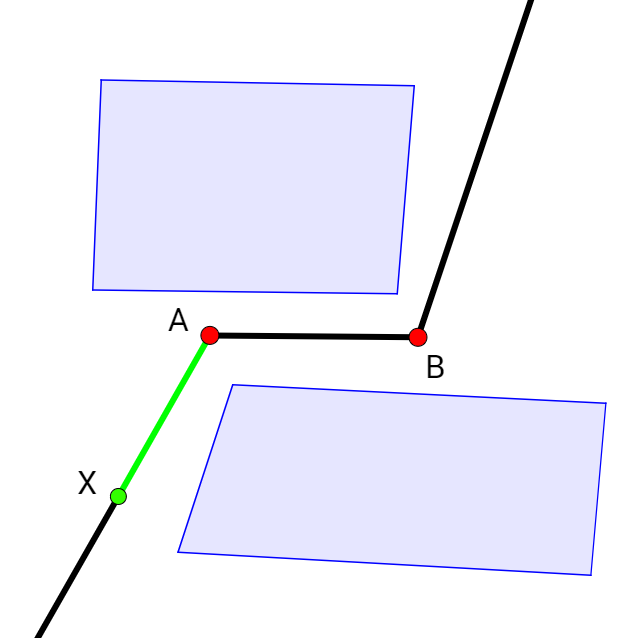
\includegraphics[width=\textwidth]{segment-xb}
        		\caption{}
        		 \label{fig:segment-demo-x}
	\end{subfigure}	
	\hfill
	\begin{subfigure}[t]{0.3\columnwidth}
        		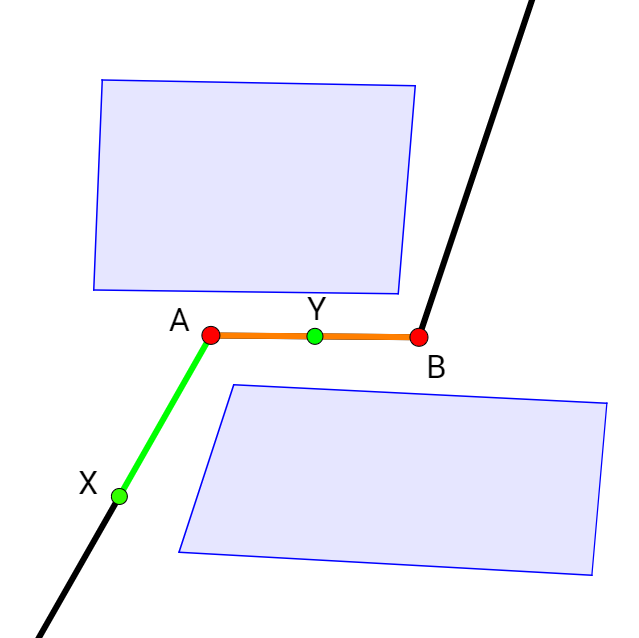
\includegraphics[width=\textwidth]{segment-yb}
        		\caption{}
        		 \label{fig:segment-demo-y}
	\end{subfigure}	
		\hfill
	\begin{subfigure}[t]{0.3\columnwidth}
        		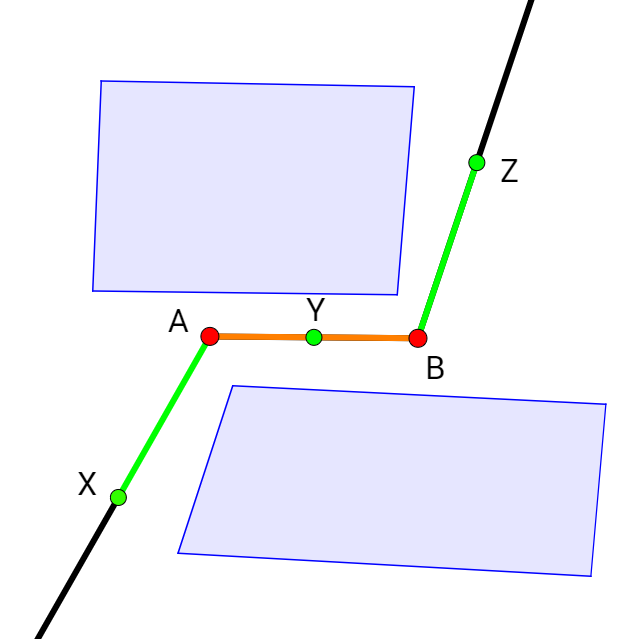
\includegraphics[width=\textwidth]{segment-z}
        		\caption{}
        		 \label{fig:segment-demo-z}
	\end{subfigure}	
	\caption[A demonstration of the segmentation algorithm]{A demonstration of the segmentation algorithm. In this example, there are two turn events at A and B as shown in red. The last segment before turn event A ends in point X, which is one expansion distance away from A. This expansion distance is marked as the green line as seen in \ref{fig:segment-demo-x}. The start position of the segment around A is X. The next step is to determine the end position of this segment. Turn event B is closer to A than the expansion distance, so the mid-point Y between A and B is chosen. This is shown in \ref{fig:segment-demo-y}, where the orange lines denote that Y is the mid-point between A and B. The segment around A is now fully constructed, starting at X and ending at Y. The next segment, around turn event B, starts in Y. There is plenty of space between B and the next turn event, so the end of the segment can be the full expansion distance removed away B, at point Z. This can be seen in \ref{fig:segment-demo-z}. The segment around B is now also fully defined, starting in Y and ending in Z. The algorithm will need to catch up to the next turn event. It will do this by adding additional straight segments which end one expansion distance before the next turn event. This leads to the situation seen in \ref{fig:segment-demo-x} as the process repeats itself.}
    \label{fig:segment-demo}     
\end{figure}

\subsection{Amount of time steps}
The amount of time steps in the MILP problem needs to be determined ahead of time. The length of the Theta* path is used to estimate how much time is needed for the UAV to reach the end of each segment. To ensure that there are always enough time steps, a conservative estimate is used. This estimate assumes that the UAV starts the segment while stopped. Afterwards, the UAV accelerates towards the turn in the segment and comes to a stop at the turn. Finally, the UAV accelerates again from the turn and stops again at the end of the segment. The time needed to complete those actions is multiplied by a multiplier parameter.

\clearpage

\section{Generating the active region for each segment}
The last step of preprocessing determines which obstacles will be modeled in the MILP problem for each segment. Segmentation already reduces the amount of time steps needed in each segment. However, modeling a large amount of obstacles still reduces the performance to unacceptable levels. \\
Not every obstacle needs to be modeled in the MILP subproblems to avoid collisions. Only the obstacles in the neighborhood around each segment are relevant. \\
Furthermore, not all obstacles in the neighborhood actually need to be modeled either. There is a fundamental difference between the obstacles on the inside of the turn and those on the outside. Obstacles on the inside of a turn are the cause for that turn. They cause the non-convex search space. Without those obstacles, the UAV could move in a straight line from the start of a segment to the goal. Therefore, obstacle avoidance for the inner obstacles must make the search space more non-convex\\
The same is not true for obstacles on the outside of the turn. Without those obstacles the optimal trajectory may have a slightly different shape, but the turn would still be there. As a result, obstacle avoidance for the outer obstacles does not necessarily have to reduce convexity. \\

\begin{figure}[h]
	\centering
	\begin{subfigure}[t]{0.45\columnwidth}
        		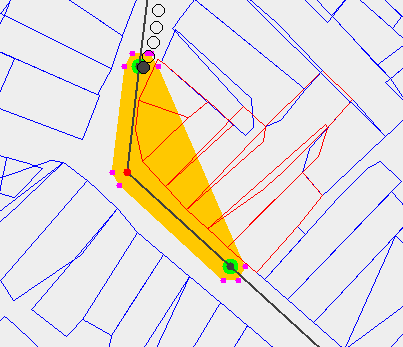
\includegraphics[width=\textwidth]{ga-seed}
        		\caption{}
        		 \label{fig:ga-seed}
	\end{subfigure}	
	\hfill
	\begin{subfigure}[t]{0.45\columnwidth}
        		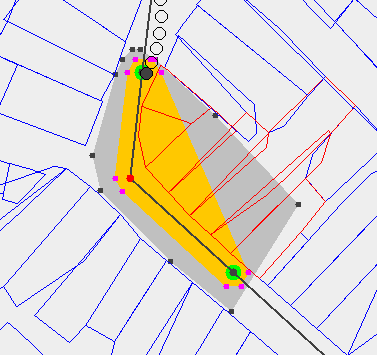
\includegraphics[width=\textwidth]{ga-seed-expanded}
        		\caption{}
        		 \label{fig:ga-seed-expanded}
	\end{subfigure}		
	\caption[A demonstration of the input and output of the genetic algorithm]{\ref{fig:ga-seed} shows the original safe region based on the convex hull of the path in orange. The obstacles that intersect this safe region are marked in red. \ref{fig:ga-seed-expanded} shows the expanded safe region as generated by the genetic algorithm in dark grey. This expanded region may not intersect any of the blue obstacles.}
    \label{fig:ga-seed-demo}     
\end{figure}

Figure \ref{fig:ga-seed} shows this difference. The obstacles on the inside of the turn are displayed in red. These are the obstacles that prevent the UAV from moving in a straight line to its goal. The other obstacles, as displayed in blue, do not prevent the UAV from moving in a straight line. As long as the UAV stays inside the orange shape, it cannot collide with any of the blue obstacles. Only the red obstacle still pose a risk. These are the obstacles that will be modeled in the MILP problem.
\par
The orange shape determines which obstacles need to be modeled. This shape is based on several important points in the segment. These points include the start position of the UAV, the goal position, and every node on the Theta* path inside the segment. Because the UAV has a physical size, these points are actually represented by regular polygons which approximate the shape of the UAV. Afterwards, the convex hull of these points/polygons is calculated using the QuickHull algorithm by Barber et al. \cite{Barber1996}. Finally, the convex hull is scale up slightly to also catch some potentially very restricting obstacles on the outside of the corner.
\par
The convex hull can be considered a safe region. If the UAV stays inside this region, it cannot collide with obstacles since any obstacle that overlaps with the safe region is modeled in the MILP problem. However, this safe region restricts the movements of the UAV more than necessary. \\
To make the safe region less restrictive, A genetic algorithm is used which attempts to expand the safe region. An example of an expanded safe region is shown in \ref{fig:ga-seed-expanded}.

\begin{algorithm}[h]
\caption{Genetic Algorithm}
\label{alg:ga}
\begin{algorithmic}[1]
\Function{GenSafeRegion}{$scenario$, $segment$}
\State $pop \leftarrow $ \Call{SeedPopulation}{}
\For {$i \gets 0, N_{gens} $}
\State $pop \leftarrow pop \cup $ \Call{Mutate}{$pop$}
\State \Call{Evaluate}{$pop$}
\State $pop \leftarrow $ \Call{Select}{$pop$}
\EndFor
\Return \Call{BestIndividual}{$pop$}
\EndFunction
\Function{Mutate}{$pop$}
\ForEach {$individual \in pop$}
\State add vertex with prob. P(add vertex)
\State OR remove vertex with prob. P(remove vertex)
\ForEach {$gene \in individual.chromosome$}
\State randomly nudge  vertex
\If{new polygon is legal}
\State update polygon
\Else
\State try again at most $N_{attempts}$ times
\EndIf
\EndFor
\EndFor
\Return \Call{BestIndividual}{$pop$}
\EndFunction
\end{algorithmic}
\end{algorithm}

\subsection{Implementation of the genetic algorithm}
A genetic algorithm is an algorithm which evolves solutions using a process inspired by natural selection in biological evolution. Genetic algorithms typically use a population of individuals which compete with each other. Each individual has a genome consisting of chromosomes, which in turn consists of individual genes. The genome determines the traits of each individual, also called the phenotype. The structure and quantity of the genes depend on the kind of problem that the genetic algorithm should solve. \\
Like in biology, the individuals can produce offspring. This offspring can be a crossover between multiple parent individuals, or a mutated version of a single parent. An important part of evolution is the concept of "survival of the fittest". A genetic algorithm improves its population by letting individuals compete. The losing individuals get eliminated from the population, while those who survive get the opportunity to create offspring. This competition is based on a fitness function. Each individual represents a possible solution for a problem. The fitness function scores the individuals based on how well they solved the problem.
\par
Algorithm \ref{alg:ga} shows the implementation of the genetic algorithm. In this implementation, each individual in the population represents a single legal polygon. A legal polygon is convex, does not self-intersect, can only overlap with the selected obstacles and contains the original safe region entirely. The latter requirement prevents the polygon from drifting off. Each individual has a single chromosome, and each chromosome has a varying number of genes. Each gene represents a vertex of the polygon.
\par
\begin{figure}[h]
\centering
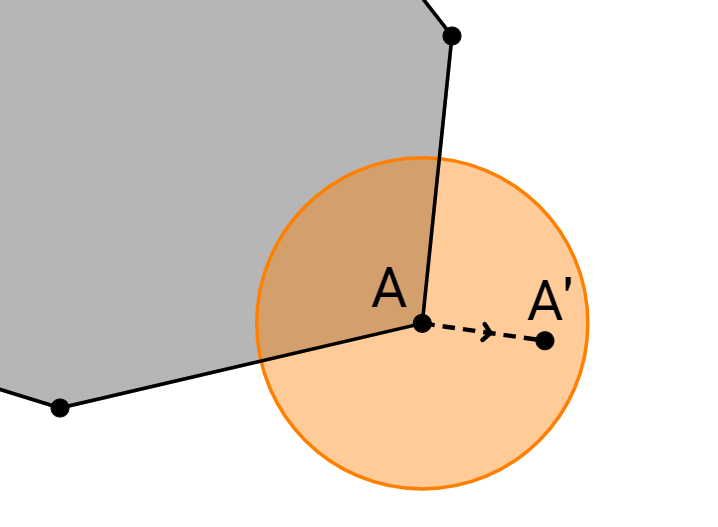
\includegraphics[width=0.45\textwidth]{genetic-mutate}
\caption[A visualization of the mutator of the genetic algorithm]{A visualization of the mutator of the genetic algorithm. The grey are is the polygon defined by the current individual. Vertex A of the individual is being mutated. The orange circle shows the maximum nudge distance. The position of the nudged vertex A' is picked at random inside this circle.}
\label{fig:genetic-mutate}
\end{figure}
The only operator is a mutator (line 4). Contrary to how mutators usually work, the mutation does not change the original individual. This means that the every individual can be mutated in every generation, since there is no risk of losing information. This mutator can add or remove vertices of the polygon by adding or removing genes (lines 12-13), but only if the amount of genes stays between a specified minimum and maximum. The mutator attempts to "nudge" every vertex/gene to a random position inside a circle around the current position (line 15). If the resulting polygon is not legal, it retries a limited number of times (line 16-19). Figure \ref{fig:genetic-mutate} shows a visual representation of this.
Tournament selection is used as the selector, with the fitness function being the surface area of the polygon (line 5-6). In tournament selection, individual compete two-by-two in each round. If an individual wins, it advances to the next round of the tournament to compete again. This is repeated until the desired population size is reached.

